% !Mode:: "TeX:DE:UTF-8:Main"
% arara: pdflatex
% arara: pdflatex
% xarara: convert: {density: 160, otheroptions: -dispose previous -delay 10 -loop 0, format: gif}
%magick -density 160 -delay 15 -loop 0 choir.pdf choir.gif
\documentclass{beamer}

\usepackage{tikzlings}
\usepackage{tikzducks,xfp}
\usetikzlibrary{overlay-beamer-styles}
\setbeamertemplate{navigation symbols}{}
\tikzset{
  mouse/.pic = {
   \begin{scope}[scale=0.5,transform shape]
     \mouse;
     \draw[black,line width=1pt](0,0.5)--(0,1);
  \end{scope}},
  }
\begin{document}
\foreach\npages in {1,2,...,500}{%
\begin{frame}<1->[plain]%%%%%%%%%%%%%%%%%%%%%%%%%%%%%%%%%%%%%%%%%%%%%%%%%
%https://scontent-lga3-1.cdninstagram.com/v/t51.2885-15/sh0.08/e35/c0.179.1440.1440a/s640x640/72792900_429534301289156_8854185985714446755_n.jpg?_nc_ht=scontent-lga3-1.cdninstagram.com&_nc_cat=108&oh=ceebf34437913589406dcce328bdeb8c&oe=5E67E95D

\begin{tikzpicture}[remember picture,overlay]
% Background image
\node[anchor=south,at={([yshift=-0.1cm]current page.south)}]{%
   \fbox{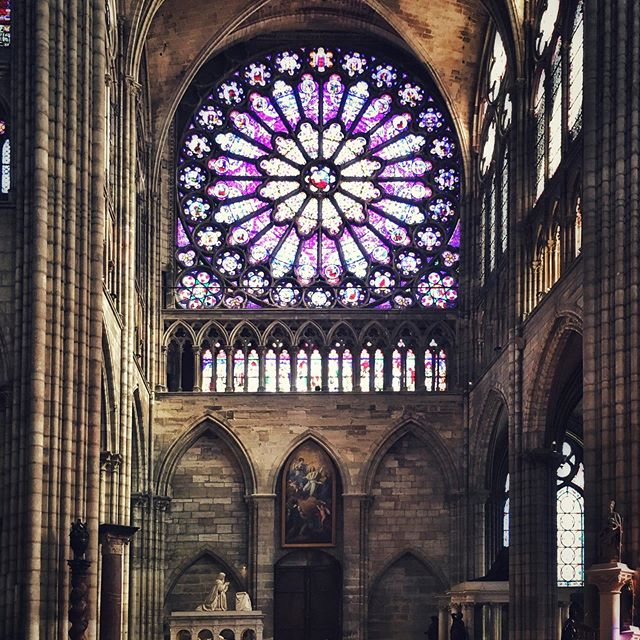
\includegraphics[height=\paperheight,trim=0cm 6cm 0cm 0cm]{rosette1}}
};	
\node[anchor=south,at={([yshift=0.31\paperheight]current page.south)}]{%
   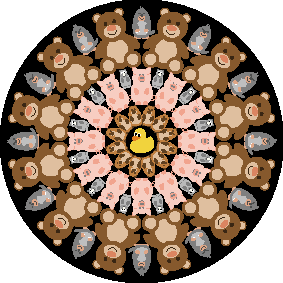
\includegraphics[height=0.6\paperheight]{mandala}
};	

\node[anchor=south,at={([yshift=0.33\paperheight,xshift=-2.5cm]current page.south)}]{%
   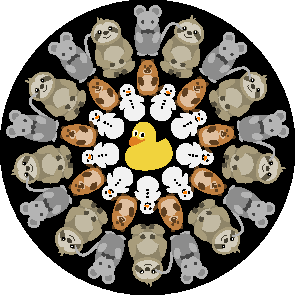
\includegraphics[height=0.1\paperheight]{mandala2}
};	
\node[anchor=south,at={([yshift=0.33\paperheight,xshift=2.4cm]current page.south)}]{%
   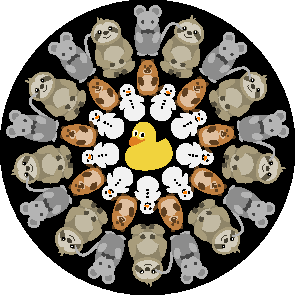
\includegraphics[height=0.1\paperheight]{mandala2}
};	

% Image credit of background
%\node[at=(current page.south east),xshift=-6.6cm,yshift=0.2cm]{%
%	\TINY\color{white}© xxxx
%};
\end{tikzpicture}

\vspace*{6.3cm}
\hspace*{\dimexpr 2.5cm+ \fpeval{5*(0.02*sin(\npages/120*4*pi))}cm}

\begin{tikzpicture}[overlay,baseline={(0,0)}]
\path (0,0) pic[scale=1.1]{mouse}--++(1,0) pic[scale=0.95]{mouse}--++(1,0) pic{mouse}--++(1,0) pic[scale=0.98]{mouse}--++(1,0) pic[scale=1.15]{mouse}--++(1,0) pic[scale=1.18]{mouse}; %--++(1,0) pic{mouse}--++(1,0) pic{mouse}--++(1,0) pic{mouse}--++(1,0) pic{mouse};
\end{tikzpicture}

\end{frame}}
\end{document}
 